\section{Zweitore - Vierpoltheorie}
\subsection{Zweitorgleichungen}
% \includegraphics[width=\columnwidth]{Zweitorgleichungen}
\begin{mdframed}[style=exercise]
    \begin{itemize}
        \item{Admittanzform/ Admittanzmatrix \textbf{Y}:}
        \begin{align*}
            \begin{split}
                \underline{I}_1 &= \underline{Y}_{11}\cdot\underline{U}_1 + \underline{Y}_{12}\cdot\underline{U}_2\\
                \underline{I}_2 &= \underline{Y}_{21}\cdot\underline{U}_1 + \underline{Y}_{22}\cdot\underline{U}_2
            \end{split}
        \left\} \
            \begin{pmatrix}
                \underline{I}_1 \\
                \underline{I}_2
            \end{pmatrix} = \textbf{\underline{Y}}\cdot
            \begin{pmatrix}
                \underline{U}_1 \\
                \underline{U}_2
            \end{pmatrix}
        \right.
        \end{align*}
        \item{Impedanzform/ Impedanzmatrix \textbf{Z}:}
            \begin{align*}
                \begin{split}
                \underline{U}_1 &=\underline{Z}_{11}\cdot\underline{I}_1 + \underline{Z}_{12}\cdot\underline{I}_2 \\
                \underline{U_2} &=\underline{Z}_{21}\cdot\underline{I}_1 + \underline{Z}_{22}\cdot\underline{I}_2
                \end{split}
            \left\} \
                \begin{pmatrix}
                    \underline{U}_1 \\
                    \underline{U}_2
                \end{pmatrix} = \textbf{\underline{Z}}\cdot
                \begin{pmatrix}
                    \underline{I}_1 \\
                    \underline{I}_2
                \end{pmatrix}
            \right.
            \end{align*}
        \item{Hybridform 1/ Reihenparallelmatrix \textbf{H}:}
            \begin{align*}
                \begin{split}
                    \underline{U}_1 &= \underline{H}_{11}\cdot\underline{I}_1 + \underline{H}_{12}\cdot\underline{U}_2 \\
                    \underline{I}_2 &= \underline{H}_{21}\cdot\underline{I}_1 + \underline{H}_{22}\cdot\underline{U}_2
                \end{split}
            \left\} \
                \begin{pmatrix}
                    \underline{U}_1 \\
                    \underline{I}_2
                \end{pmatrix} = \textbf{\underline{H}}\cdot
                \begin{pmatrix}
                    \underline{I}_1 \\
                    \underline{U}_2
                \end{pmatrix}
            \right.
            \end{align*}
            \item{Hybridform 2/ Parallelreihenmatrix \textbf{C}:}
            \begin{align*}
                \begin{split}
                    \underline{I}_1 &= \underline{C}_{11}\cdot\underline{U}_1 + \underline{C}_{12}\cdot\underline{I}_2 \\
                    \underline{U}_2 &= \underline{C}_{21}\cdot\underline{U}_1 + \underline{C}_{22}\cdot\underline{I}_2
                \end{split}
            \left\} \
                \begin{pmatrix}
                    \underline{I}_1 \\
                    \underline{U}_2
                \end{pmatrix} = \textbf{\underline{C}}\cdot
                \begin{pmatrix}
                    \underline{U}_1 \\
                    \underline{I}_2
                \end{pmatrix}
            \right.
            \end{align*}
            \item{Kettenform/ Kettenmatrix \textbf{A}:}
                \begin{align*}
                    \begin{split}
                        \underline{U}_1 &= \underline{A}_{11}\cdot\underline{U}_2 + \underline{A}_{12}\cdot-\underline{I}_2 \\
                        \underline{I}_1 &= \underline{A}_{21}\cdot\underline{U}_2 + \underline{A}_{22}\cdot-\underline{I}_2
                    \end{split}
                \left\} \
                    \begin{pmatrix}
                        \underline{U}_1 \\
                        \underline{I}_2
                    \end{pmatrix} = \textbf{\underline{A}}\cdot
                    \begin{pmatrix}
                        \underline{U}_2 \\
                        -\underline{I}_2
                    \end{pmatrix}
                \right.
                \end{align*}
                \item{Kettenform rückwärts/ Kettenmatrix \textbf{B}:}
                    \begin{align*}
                        \begin{split}
                            \underline{U}_2 &= \underline{B}_{11}\cdot\underline{U}_1 + \underline{B}_{12}\cdot-\underline{I}_1\\
                            \underline{I}_2 &= \underline{B}_{21}\cdot\underline{U}_1 + \underline{B}_{22}\cdot-\underline{I}_1
                        \end{split}
                    \left\} \
                    \begin{pmatrix}
                        \underline{U}_2\\
                        \underline{I}_2
                    \end{pmatrix} = \textbf{\underline{B}}\cdot
                    \begin{pmatrix}
                        \underline{U}_1 \\
                        -\underline{I}_1
                    \end{pmatrix}
                \right.
                    \end{align*}
    \end{itemize}
\end{mdframed}

\subsubsection{Parameterumrechnung}
\begingroup
\arraycolsep=1.0pt\def\arraystretch{2.0}
\begin{align*}
    Z && \hspace{0.5cm} Y && \hspace{0.5cm} H && \hspace{0.5cm} A
\end{align*}
\[
    Z\
    \begin{bmatrix}
        \underline{Z}_{11} & \underline{Z}_{12}\\
        \underline{Z}_{21} & \underline{Z}_{22}
    \end{bmatrix}
    \begin{bmatrix}
        \dfrac{\underline{Y}_{22}}{\operatorname{det}\underline{\boldsymbol{Y}}} & \dfrac{-\underline{Y}_{12}}{\operatorname{det} \underline{\boldsymbol{Y}}}\\
        \dfrac{-\underline{Y}_{21}}{\operatorname{det} \underline{\boldsymbol{Y}}} & \dfrac{\underline{{Y}}_{11}}{\operatorname{det} \underline{\boldsymbol{Y}}} \\
    \end{bmatrix}
    \begin{bmatrix}
        \dfrac{\operatorname{det}\underline{\boldsymbol{{H}}}}{\underline{H}_{22}} & \dfrac{\underline{H}_{12}}{\underline{H}_{22}} \\
        \dfrac{-\underline{H}_{21}}{\underline{H}_{22}} & \dfrac{1}{\underline{H}_{22}}
    \end{bmatrix}
    \begin{bmatrix}
        \dfrac{\underline{A}_{11}}{\underline{A}_{21}} & \dfrac{\operatorname{det}\underline{\boldsymbol{A}}}{\underline{A}_{21}}\\
        \dfrac{1}{\underline{A}_{21}} & \dfrac{\underline{{A}}_{22}}{\underline{A}_{21}} \\
    \end{bmatrix}
\]
\[
    Y\
    \begin{bmatrix}
        \dfrac{\underline{Z}_{22}}{\operatorname{det}\underline{\boldsymbol{Z}}} & \dfrac{-\underline{Z}_{12}}{\operatorname{det} \underline{\boldsymbol{Z}}}\\
        \dfrac{-\underline{Z}_{21}}{\operatorname{det} \underline{\boldsymbol{Z}}} & \dfrac{\underline{{Z}}_{11}}{\operatorname{det} \underline{\boldsymbol{Z}}} \\
    \end{bmatrix}
    \begin{bmatrix}
        \underline{Y}_{11} & \underline{Y}_{12}\\
        \underline{Y}_{21} & \underline{Y}_{22}
    \end{bmatrix}
    \begin{bmatrix}
        \dfrac{1}{\underline{H}_{11}} & \dfrac{-\underline{H}_{12}}{\underline{H}_{11}} \\
        \dfrac{\underline{H}_{21}}{\underline{H}_{11}} & \dfrac{\operatorname{det}\underline{\boldsymbol{{H}}}}{\underline{H}_{11}}
    \end{bmatrix}
    \begin{bmatrix}
        \dfrac{\underline{A}_{22}}{\underline{A}_{12}} & \dfrac{-\operatorname{det}\underline{\boldsymbol{A}}}{\underline{A}_{12}}\\
        \dfrac{-1}{\underline{A}_{12}} & \dfrac{\underline{{A}}_{11}}{\underline{A}_{12}} \\
    \end{bmatrix}
\]
\[
    H\
    \begin{bmatrix}
        \dfrac{\operatorname{det}\underline{\boldsymbol{{Z}}}}{\underline{Z}_{22}} & \dfrac{\underline{Z}_{12}}{\underline{Z}_{22}} \\
        \dfrac{-\underline{Z}_{21}}{\underline{Z}_{22}} & \dfrac{1}{\underline{Z}_{22}}
    \end{bmatrix}
    \begin{bmatrix}
        \dfrac{1}{\underline{Y}_{11}} & \dfrac{-\underline{Y}_{12}}{\underline{Y}_{11}} \\
        \dfrac{\underline{Y}_{21}}{\underline{Y}_{11}} & \dfrac{\operatorname{det}\underline{\boldsymbol{{Y}}}}{\underline{Y}_{11}}
    \end{bmatrix}
    \begin{bmatrix}
        \underline{H}_{11} & \underline{H}_{12}\\
        \underline{H}_{21} & \underline{H}_{22}
    \end{bmatrix}
    \begin{bmatrix}
        \dfrac{\underline{A}_{12}}{\underline{A}_{22}} & \dfrac{\operatorname{det}\underline{\boldsymbol{A}}}{\underline{A}_{22}}\\
        \dfrac{-1}{\underline{A}_{22}} & \dfrac{\underline{{A}}_{21}}{\underline{A}_{22}} \\
    \end{bmatrix}
\]
\[
    A\
    \begin{bmatrix}
        \dfrac{\underline{Z}_{11}}{\underline{Z}_{21}} & \dfrac{\operatorname{det}\underline{\boldsymbol{Z}}}{\underline{Z}_{21}}\\
        \dfrac{1}{\underline{Z}_{21}} & \dfrac{\underline{{Z}}_{22}}{\underline{Z}_{21}} \\
    \end{bmatrix}
    \begin{bmatrix}
        \dfrac{-\underline{Y}_{22}}{\underline{Y}_{21}} & \dfrac{-1}{\underline{Y}_{21}}\\
        \dfrac{-\operatorname{det}\underline{\boldsymbol{Y}}}{\underline{Y}_{21}} & \dfrac{-\underline{{Y}}_{11}}{\underline{Y}_{21}} \\
    \end{bmatrix}
    \begin{bmatrix}
        \dfrac{-\operatorname{det}\underline{\boldsymbol{{H}}}}{\underline{H}_{21}} & \dfrac{-\underline{H}_{11}}{\underline{H}_{21}} \\
        \dfrac{-\underline{H}_{22}}{\underline{H}_{21}} & \dfrac{-1}{\underline{H}_{21}}
    \end{bmatrix}
    \begin{bmatrix}
        \underline{A}_{11} & \underline{A}_{12}\\
        \underline{A}_{21} & \underline{A}_{22}
    \end{bmatrix}
\]
\endgroup

% \includegraphics[width=\columnwidth,height=9cm]{Parameterumrechnung}\\

\subsection{Zusammenschalten von Zweitoren}

\begin{mdframed}[style=exercise]
\begin{itemize}
    \item Reihenschaltung:
        \begin{center}
            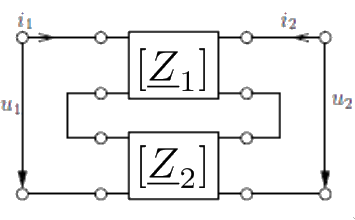
\includegraphics[width=0.5\textwidth]{Reihenschaltung_Zweitore}
        \[
            \left[ \underline{Z} \right] = \left[ \underline{Z}_1 \right] + \left[ \underline{Z}_2 \right]
        \]
        \end{center}
    \item Parallelschaltung:
        \begin{center}
            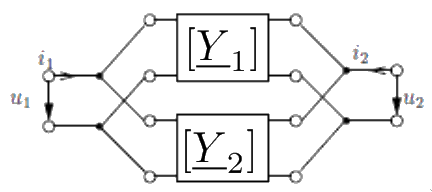
\includegraphics[width=0.6\textwidth]{Parallelschaltung_Zweitoren}
        \[
            \left[ \underline{Y} \right] = \left[ \underline{Y}_1 \right] + \left[ \underline{Y}_2 \right]
        \]
        \end{center}
    \item Kettenschaltung:
        \begin{center}
            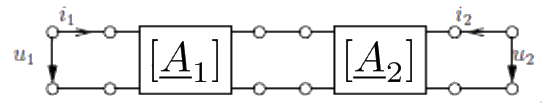
\includegraphics[width=0.7\textwidth]{Kettenschaltung_Zweitoren}
        \[
            \left[ \underline{A} \right] = \left[ \underline{A}_1 \right] \cdot \left[ \underline{A}_2 \right]
        \]
        \end{center}
        \footnotesize
        \textsc{Beachte:}\\
        \normalsize Im Allgemeinen gilt $\rightarrow
        \left[ \underline{A}_1 \right] \cdot \left[
        \underline{A}_2 \right] \neq \left[ \underline{A}_2
        \right] \cdot \left[ \underline{A}_1 \right]$
    \item Reihen-Parallelschaltung:
        \begin{center}
            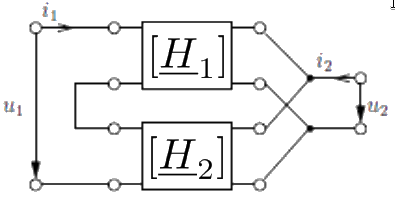
\includegraphics[width=0.5\textwidth]{Reihen-Parallelschaltung_Zweitoren}
        \[
            \left[ \underline{H} \right] = \left[ \underline{H}_1 \right] \cdot \left[ \underline{H}_2 \right]
        \]
        \end{center}
    \item Parallel-Reihenschaltung:
        \begin{center}
            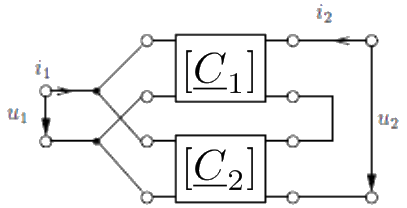
\includegraphics[width=0.5\textwidth]{Parallel-Reihenschaltung_Zweitoren}
        \[
            \left[ \underline{C} \right] = \left[ \underline{C}_1 \right] \cdot \left[ \underline{C}_2 \right]
        \]
        \end{center}
\end{itemize}
\end{mdframed}


\begin{samepage}
    \onecolumn
    \subsection{Matrizen elementarer Zweitore}
    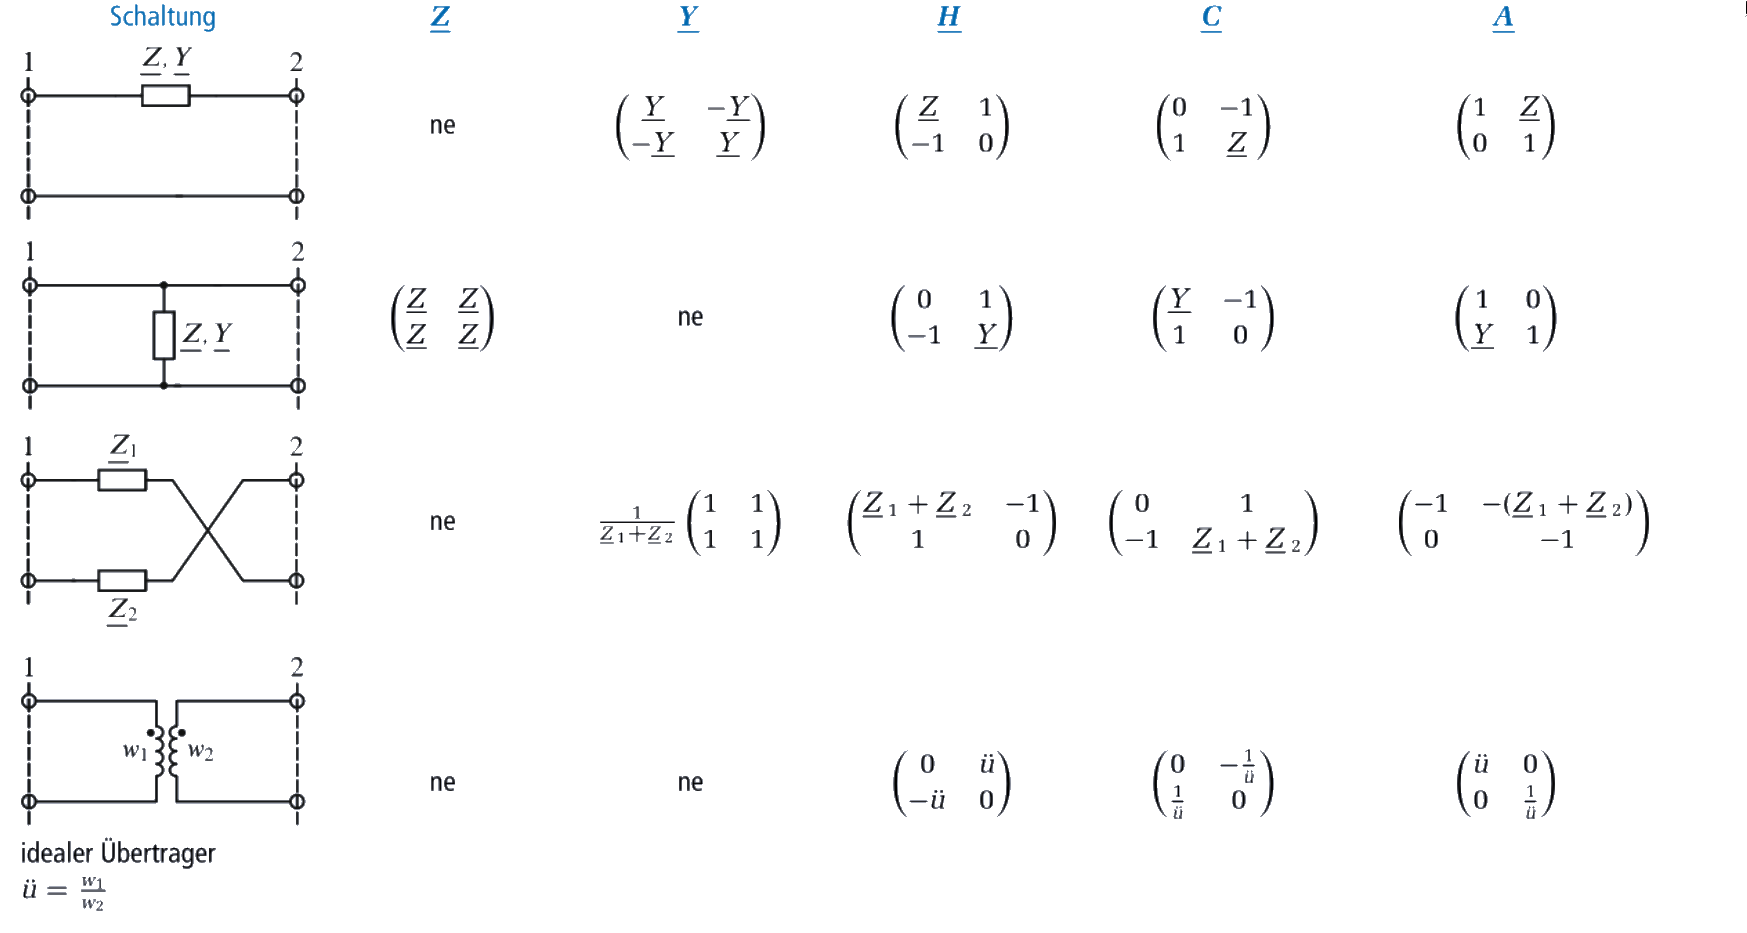
\includegraphics[width=\columnwidth]{converted/Matrizen_elementarer_zweitore}
    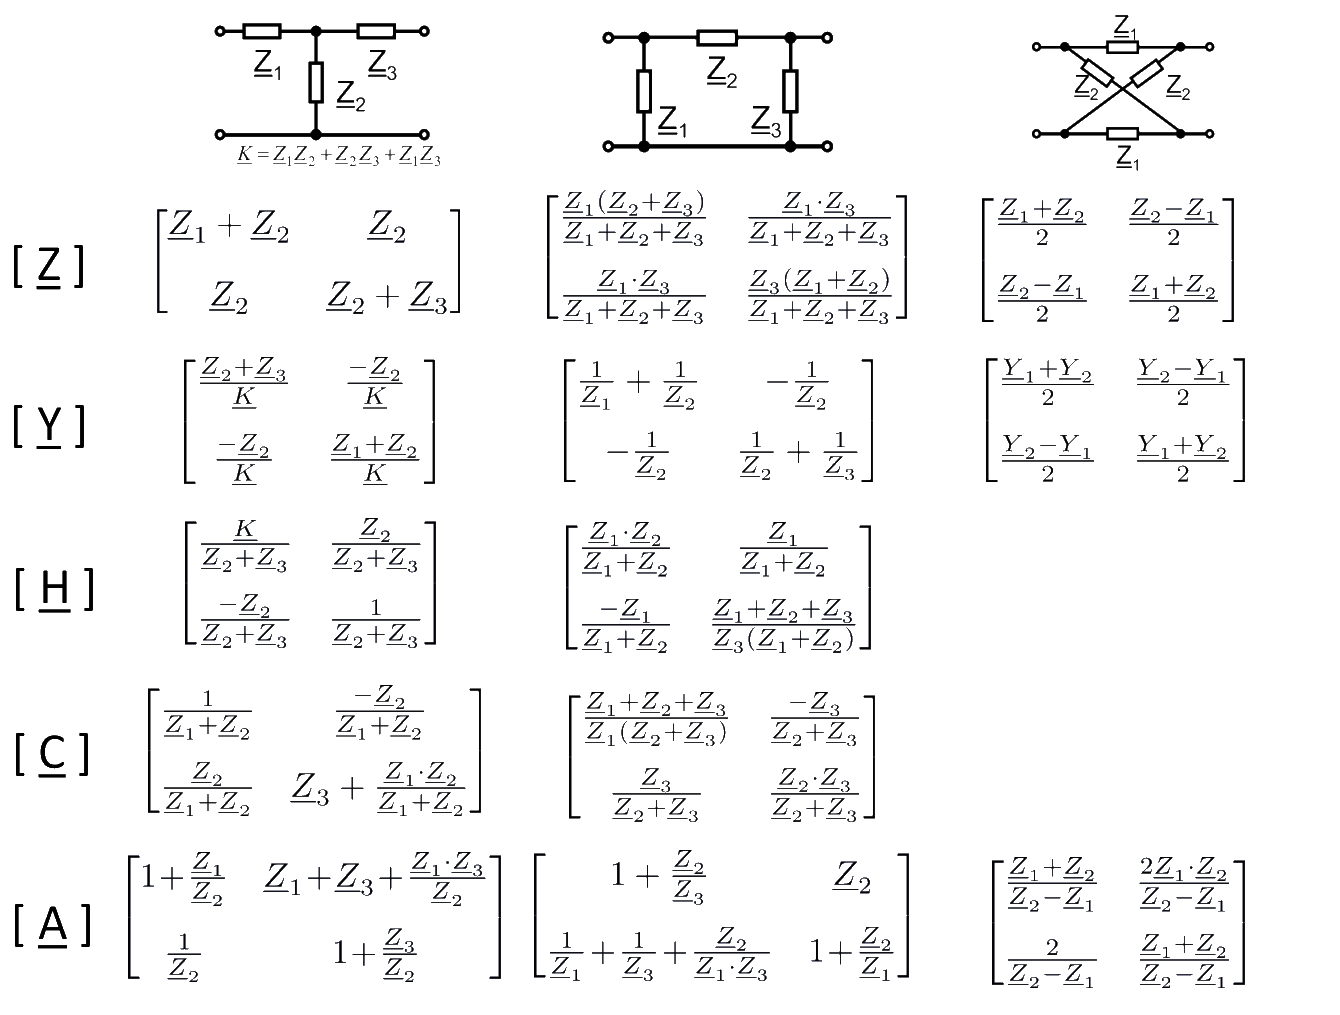
\includegraphics[width=\columnwidth]{converted/Matrizen_elementarer_zweitore_1}
\end{samepage}
\twocolumn

\subsubsection{Trennverst\"arker}
\begin{mdframed}[style=exercise]
Ersatzschaltbild eines idealen Trennverst\"arkers:
    \begin{center}
        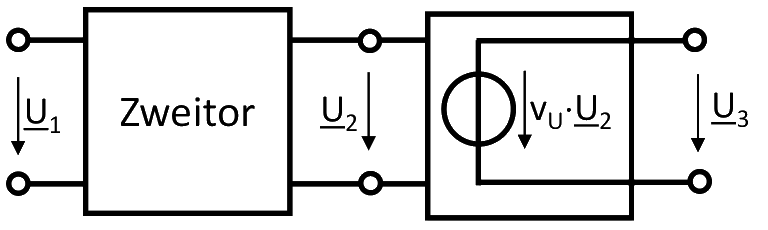
\includegraphics[width=0.7\textwidth]{Trennverstaerker_esb}
    \end{center}
    \[
        A = \begin{pmatrix}
            \dfrac{1}{v_U} & 0 \\
                  0        & 0
        \end{pmatrix}
    \]
    \[
        \underline{A}_e = \begin{pmatrix}
            \underline{A}_{11} & \underline{A}_{12}\\
            \underline{A}_{21} & \underline{A}_{22}
        \end{pmatrix}
        \cdot
        \begin{pmatrix}
            \dfrac{1}{v_U} & 0 \\
                  0        & 0
        \end{pmatrix}
        = \begin{pmatrix}
            \dfrac{\underline{A}_{11}}{v_U} & 0\\
            \dfrac{\underline{A}_{21}}{v_U} & 0
        \end{pmatrix}
    \]
\end{mdframed}

\subsubsection{Torbedingungen}
Die Torbedingungen werden durch:
    \begin{itemize}
        \item idealen \"Ubertrager
        \item Kurzschlussschleife
        \item Parallelschaltung längssymmetrischer Zweitore
    \end{itemize} erf\"ullt.


für die das Zusammenschalten von Zweitoren müssen diese Bedingungen
eingehalten werden.

\subsection{Zweitor Eigenschaften:}
\begin{itemize}
        % \setlength{\itemindent}{-1em}
    \item Reziprozit\"at (Umkehrbarkeit)
        \begin{center}
            \begin{tabular}{|c|c|}
                \hline
                $Z$&  $Z_{12} = Z_{21}$\\
                \hline
                $Y$&  $Y_{12} = Y_{21}$\\
                \hline
                $A$&  $\operatorname{det}[A] = 1$\\
                \hline
                $H$&  $H_{12} = -H_{21}$\\
                \hline
            \end{tabular}
        \end{center}
        Ein umkehrbares (reziprokes) Zweitor wird\\ nur durch drei Parameter
        beschrieben:

        \footnotesize
        \textbf{(RLCM-Zweitor)ist immer umkehrbar.}

        {\color{red}{Gegenbeispiel:}} idealer Transistor
        \normalsize
    \item R\"uckwirkungsfreiheit\\
        $$Z_{12}=Y_{12}=H_{12}=\operatorname{det}[A]=0$$
        Ein rückwirkungsfreies Zweitor ist nicht reziprok und wird nur durch
        drei Parameter beschrieben.\\
        \footnotesize
        Beispiele: idealer Verstärker, idealer Transistor, gesteuerte Quellen
        \normalsize
    \item Symmetrie
        \begin{center}
            \begin{tabular}{|c|c|}
                \hline
                $Z$&  $Z_{11} = Z_{22}$\\
                \hline
                $Y$&  $Y_{11} = Y_{22}$\\
                \hline
                $A$&  $A_{11} = A_{22}$\\
                \hline
                $H$&  $\operatorname{det}[H]=1$\\
                \hline
            \end{tabular}
        \end{center}
        Ein umkehrbares und symmetrisches Zweitor wird durch zwei Parameter
        beschrieben.
\end{itemize}
\newpage

\subsection{Zweitorersatzschaltung}
\subsubsection{gesteuerte Quellen}
\begin{mdframed}[style=exercise,frametitle=Ideal]
    \footnotesize
    VCVS: Spannungsgesteurte Spannungsquelle\\
    CCVS: Stromgesteurte Spannungsquelle\\
    VCCS: Spannungsgesteurte Stromquelle\\
    CCCS: Stromgesteurte Stromquelle
    \normalsize
    \begin{center}
        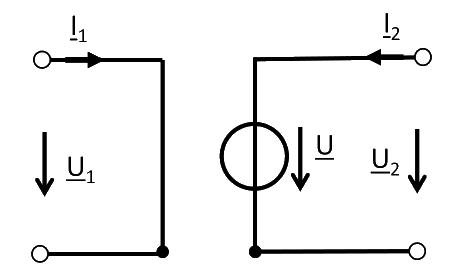
\includegraphics[width=0.5\columnwidth]{spg-spg-gestuert}\\
    \begin{tabular}{l c}
       VCVS:& $\underline{U}=\alpha\cdot \underline{U}_1$\\
       CCVS:& $\underline{U}=Z_T\cdot \underline{I}_1$\\
    \end{tabular}
    \end{center}
    \begin{center}
        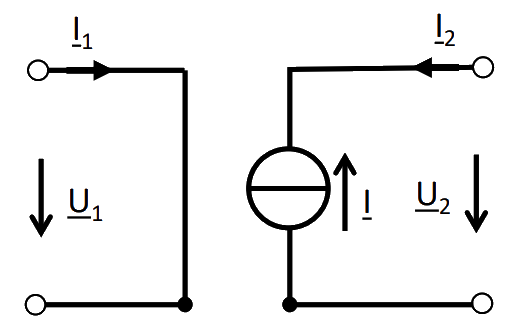
\includegraphics[width=0.45\columnwidth]{strm-strm-gesteuert}\\
    \begin{tabular}{l c}
       VCCS:& $\underline{I}=\beta\cdot \underline{I}_1$\\
       CCCS:& $\underline{I}=Y_T\cdot \underline{U}_1$\\
    \end{tabular}
    \end{center}
    Andere Matrizen sind nicht definiert.  Ideale (gesteuerte) Quellen lassen
    sich nicht ineinander umwandeln!
\end{mdframed}

\begin{mdframed}[style=exercise,frametitle=Linear]
    \begin{center}
        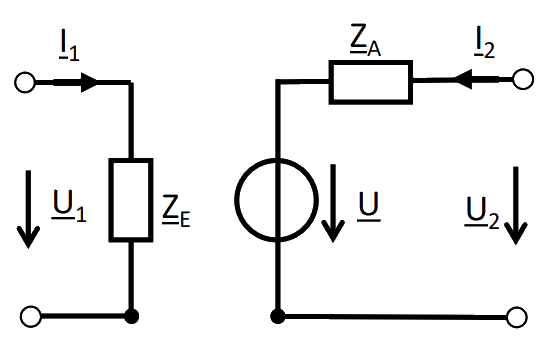
\includegraphics[width=0.5\columnwidth]{spg-spg-gestuert_linear}\\
    \begin{tabular}{l c}
        VCVS& $\underline{U}=\alpha\cdot \underline{U}_1$\\
        CCVS:& $\underline{U}=Z_T\cdot \underline{I}_1 = \alpha Z_E\cdot \underline{I}_1 $\\
    \end{tabular}
    \end{center}
    \begin{center}
        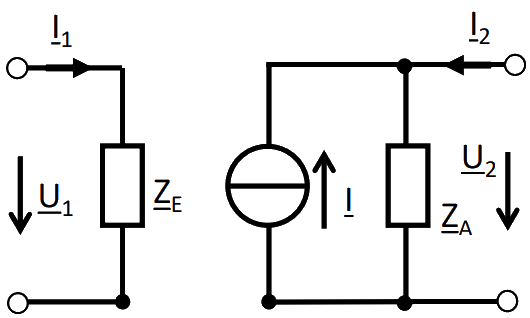
\includegraphics[width=0.47\columnwidth]{strm-strm-gesteuert_linear}\\
    \begin{tabular}{l c}
        CCVS:& $\underline{I}=\beta\cdot \underline{I}_1 = \alpha \frac{\underline{Z}_E}{\underline{Z}_{A}}\cdot \underline{I}_1$\\
        CCCS:& $\underline{I}=Y_T\cdot \underline{U}_1 = \frac{\alpha}{\underline{Z}_{A}}\cdot \underline{U}_1$\\
    \end{tabular}
    \end{center}
% /home/ayham/Downloads/1 Vierpole.pdf:29 Matrizen maybe sinnvoll
\end{mdframed}
\subsubsection{Ersatzschaltbilder}
\begin{itemize}
    \item T-Ersatzschaltbild für Z-Matrix\\
        für $Z_{12} \neq Z_{21}$ ergänzt um eine gesteuerte Quelle.\\
        \centering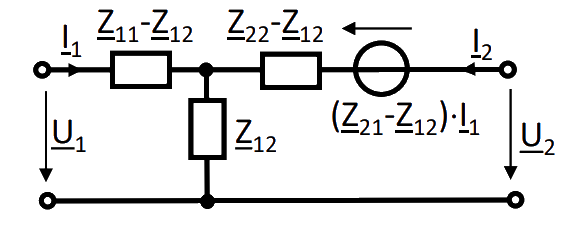
\includegraphics[width=0.7\columnwidth]{esb_t-mit_cs}

        \raggedright
    \item $\Pi$-Ersatzschaltbild für Y-Matrix\\
        für $Y_{12} \neq Y_{21}$ ergänzt um eine gesteuerte Quelle.\\
        \centering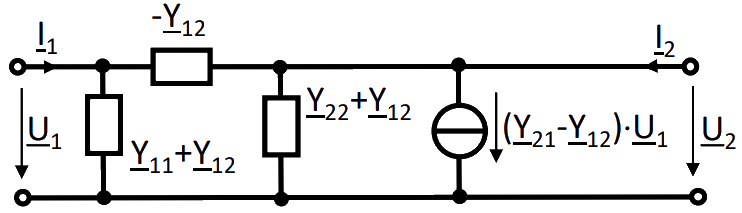
\includegraphics[width=0.8\columnwidth]{esb_pi-mit_cs}

        \raggedright
    \item  Hybrid-Ersatzschaltbild für H-Matrix\\
        \centering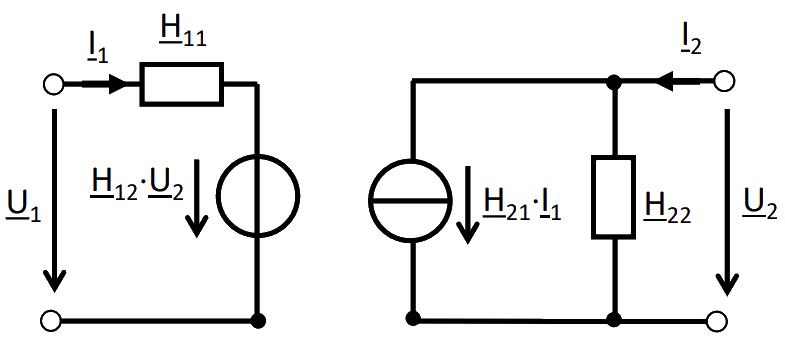
\includegraphics[width=0.7\columnwidth]{esb_hybrid-mit_cs}
\end{itemize}

\subsection{Beschaltete Zweitore}
\subsubsection{Eingangsimpedanz}
\centering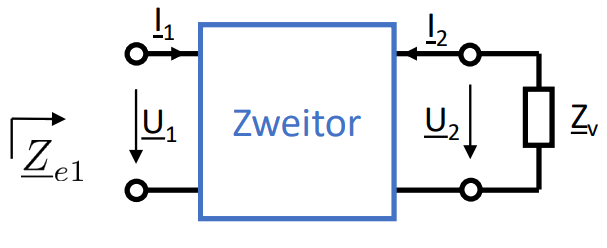
\includegraphics[width=0.5\columnwidth]{Eingangsimpedanz}
\begin{mdframed}[style=exercise]
    \begin{align*}
        \boldsymbol{Z}\rightarrow&\  \underline{Z}_{e1} = \underline{Z}_{11}-\frac{\underline{Z}_{12}\underline{Z}_{21}}{\underline{Z}_{22}+\underline{Z}_V}\\
        \boldsymbol{Y}\rightarrow&\  \underline{Y}_{e1} = \underline{Y}_{11}-\frac{\underline{Y}_{12}\underline{Y}_{21}}{\underline{Y}_{22}+\underline{Y}_V}\\
        \boldsymbol{A}\rightarrow&\  \underline{Z}_{e1} = \frac{\underline{A}_{11}\underline{Z}_V + \underline{A}_{12}}{\underline{A}_{21}\underline{Z}_V+\underline{A}_{22}}\\
        \boldsymbol{H}\rightarrow&\  \underline{Z}_{e1} = \underline{H}_{11}-\frac{\underline{H}_{12}\underline{H}_{21}}{\underline{H}_{22}+\underline{Y}_V}\\
        \boldsymbol{C}\rightarrow&\  \underline{Y}_{e1} = \underline{C}_{11}-\frac{\underline{C}_{12}\underline{C}_{21}}{\underline{C}_{22}+\underline{Z}_V}\\
    \end{align*}
\end{mdframed}
\raggedright

\subsubsection{Ausgangsimpedanz}
\centering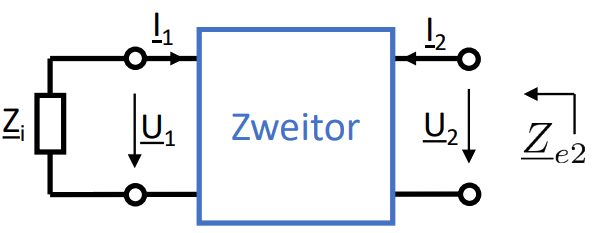
\includegraphics[width=0.5\columnwidth]{Ausgangsimpedanz}
\begin{mdframed}[style=exercise]
    \begin{align*}
        \boldsymbol{Z}\rightarrow&\  \underline{Z}_{e2} = \underline{Z}_{22}-\frac{\underline{Z}_{12}\underline{Z}_{21}}{\underline{Z}_{11}+\underline{Z}_i}\\
        \boldsymbol{Y}\rightarrow&\  \underline{Y}_{e2} = \underline{Y}_{22}-\frac{\underline{Y}_{12}\underline{Y}_{21}}{\underline{Y}_{11}+\underline{Y}_i}\\
        \boldsymbol{A}\rightarrow&\  \underline{Z}_{e2} = \frac{\underline{A}_{22}\underline{Z}_i + \underline{A}_{12}}{\underline{A}_{21}\underline{Z}_i+\underline{A}_{11}}\\
        \boldsymbol{H}\rightarrow&\  \underline{Z}_{e2} = \underline{H}_{22}-\frac{\underline{H}_{12}\underline{H}_{21}}{\underline{H}_{11}+\underline{Y}_i}\\
        \boldsymbol{C}\rightarrow&\  \underline{Y}_{e2} = \underline{C}_{22}-\frac{\underline{C}_{12}\underline{C}_{21}}{\underline{C}_{11}+\underline{Z}_i}\\
    \end{align*}
\end{mdframed}
\raggedright

\subsubsection{Ersatzquelle}
\centering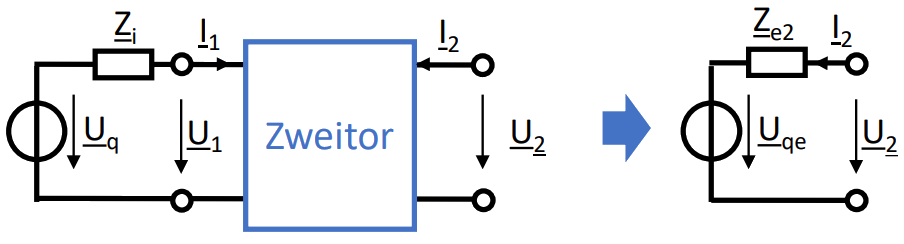
\includegraphics[width=0.7\columnwidth]{Ersatzquelle}
\begin{mdframed}[style=exercise]
    \begin{align*}
        \boldsymbol{Z}\rightarrow&\  \underline{U}_{qe} = \frac{\underline{U}_q\underline{Z}_{21}}{\underline{Z}_{11}+\underline{Z}_i}\\
        \boldsymbol{Y}\rightarrow&\  \underline{I}_{qe} = \frac{-\underline{I}_q\underline{Y}_{21}}{\underline{Y}_{11}+\underline{Y}_i}\\
        \boldsymbol{A}\rightarrow&\  \underline{U}_{qe} = \frac{\underline{U}_q}{\underline{Z}_i\underline{A}_{21}+\underline{A}_{11}}\\
        \boldsymbol{H}\rightarrow&\  \underline{I}_{qe} = \frac{-\underline{U}_q\underline{H}_{21}}{\underline{H}_{11}+\underline{Z}_i}\\
        \boldsymbol{C}\rightarrow&\  \underline{U}_{qe} = \frac{\underline{I}_q\underline{C}_{21}}{\underline{C}_{11}+\underline{Y}_i}\\
    \end{align*}
\end{mdframed}
\raggedright
